\section{Introduction}

According to the Consumer Reports, 2.1 million smartphones were stolen in the United States in 2014[1]. The Pew Internet Project reported in 2012 that nearly one third of mobile phone users have experienced a lost or stolen device [2]. Lookout estimates that phone lost could cost U.S. consumers 30 billion dollars per year [3]. Moreover, hardware loss is not the only risk of phone theft. Egelman et al. indicates that $42\%$ of users do not lock their smartphones, and this allows thieves to gain access to victims' personal information stored on their mobile devices [4]. In this paper, we present a novel method to automatically detect pick-pocket and grab-and-run smartphone theft using binary classifiers that distiguishes between theft and normal usage. \\

In order to generate a labeled data set, we carefully designed experiments that simulated three types of phone theft, grab-and-run when the user stood stills, grab-and-run while the user was moving and pick-pocket and ran 20 trials for each kind of theft. We also conducted a user study, where we tracked 55 participants for 3 weeks and collected sensor data from their smartphones. We then extracted 14 features from the raw acceleromter data to constitute the training and validation sets. Our classifiers are triggered when the norm of the accelerometer data exceeds $40m/s^2$.

We evaluated three standard machine learning algorithms: linear SVM, logistic regression and random forest. We show that for smartphone theft detection, logistic regression produces 2 false alarms per week while detecting 96.7\% theft


\section{Related Work}
\textcolor{red}{ToDo} \\


\section{Methodology}

\subsection{Data Collection}

\subsubsection{Simulated Thefts}
We carefully designed experiments to simulate three types of smartphone theft scenarios with one researcher acting as a smartphone user, and another one playing the role of a thief. In the first scenario, the user stood still and held the phone as if it was being usd, for instance texting; the thief approached from behind, grabbed the phone and ran away in the forward direction. In the second scenario, the user again held the phone in front of her while walking at a constant speed; the thief approached from behind, grabbed the phone and ran away in the forward direction. The third scenario simulated pick-pocket theft. The user placed the phone in a back pocket and stood still; the thief approached from behind, stole the phone from user's pocket and ran away in the forward direction. \\
We collected 20 instances of each of the three theft scenarios. Between two consective trials, researchers put the phone down on the ground for 30-50 seconds which created gaps to help seperate trials. We ran those three scenarios at two different times, each of which consisted of 30 trials and lasted approximately one hour. We chose to run the experiments on a flat ground at an open space, so the experiments were not be interrupted. We also made sure that the thief could run at least 40 feet after gaining possession of the victim's phone.

\textcolor{red}{Irwin's feedback; I am not sure how to address it: From a methodological standpoint, this section makes me suspect that your classifier isn't picking up on theft vs. not-theft, but rather slow vs. fast motion; do you have any analysis that addresses this?}


\subsubsection{User Study}
We conducted a user study in the Bay Area in the United States from September to December 2016 to collect smartphone sensor data, including accelerometer, step count, ambient light, etc, from participants' daily usage. The accelerometer data collected from this user study was then used to generate negative samples for the machine learning algorithms. \\
We first posted a recruitment advertisement on the Craigslist under the SF Bay Area `et cetera jobs' category in September 2016. All subjects were required to take an online screening survey, in which they provided information about their age, gender, smartphone maker and model, the way to carry a phone, e.g. in a pocket or a purse, and whether they are comfortable with wearing a smartwatch. We only recruited participants who used an Android phone with version 5.0 and above, and were willing to wear a smartwatch. \\
All qualified participants were scheduled a 30-minute meeting with a researcher. During the meeting, they were instructed to install an application on their smartphones, which collected and transmitted sensor data from their smartphones to a private account on a cloud server. All log files that contained sensor data were encrypted using AES/CCM with an 11 byte Nonce and a 16 byte MAC upon hourly upload to a cloud server. Researchers also provided each participant with a Basis Peak smartwatch and explained that they might experience overheat while wearing it, and if it did, they should take it off and contact us immediately. The watch was paired with participant's smartphone via bluetooth, and the installed app collected data that could be used to determine if the smartphone was close to the watch. We used it as the ground truth of the smartphone being in user's possession. We asked participants to wear a smartwatch for as long as possible during the study except while sleeping. At the end of the meeting, they signed a consent form, which explained the purpose, requirements, risks, confidentiality and compensation of the study. Participants then received \$25 Visa gift card. \\
During the user study, researchers contacted participants weekly to make sure that their phones and watches functioned correctly. \\
After completing the study, participants returned the watch, filled out a short exit survey and received compensation of \$125 Visa gift card. \\
We had a total of 3 rounds; each round lasted 3 consecutive weeks. A total of 55 participants were recruited. 53 out of the 55 subjects completed the study. In the first round, 16 out of 18 participants finished the study. All 18 subjects who participated in the second round completed the study. So are all 19 participants in the third round. \\
\textcolor{red}{ToDo: participants' demographic information} \\


\subsection{Feature Extraction}
We first selected a number of candidate features to evaluate, minimum, maximum, mean, standard deviation, root mean square, arc length, arc length times standard deviation, and mean absolute of the x, y, z, and magnitude of accelerometer data. Eventaully, we selected maximum, mean, standard deviation, root mean square, arc length, arc length times standard deviation, and mean absolute. And those features were computed for the magnitude of accelerometer data because compared to x, y, z accelerometer data, the magnitude is non-directional thus more robust to the orientation change and performed better. We removed minimum from the feature sets because it did not seem to provide useful infomation for the classifiers. We decided to use magnitude of accelerometer exceeding 40 $m/s^2$ as a trigger condition for our classifiers. We calculated feature vectors of one-second window before and after each 40-spike in the magnitude of the accelerometer data, so that the classifiers can capture the motion change before and after the moment when the smartphone was stolen. As a result, we generated 60 positive data points and 248508 negative data points. Each data point is a 12 dimentsional feature vector.


\subsection{Machine Learning Algorithms}
We evaluated three standard machine learning algorithms: logistic regression , random forest and linear SVM, provide by the Python scikit-learn library, to distinguish between theft and normal usage. In order to mitigate the fact we have much more negative samples than the positive ones, we set the class weight class attribute built in the library to `balanced,' which adjusts the class weights to be inversely proportional to class frequencies in the input data.


\section{Results}
We ran a 10-fold cross validation on the entire data set, which consisted of 60 positive samples and 248385 negative samples. Among the three machine learning algorithms chosen, logistic regression performs the best in term of lowest false negative and false positive rate. Confusion matrices of logistic regression, random forest and linear SVM are shown as comparisons, \\

\begin{tabular}{l|l|c|c|}
\multicolumn{2}{c}{} &\multicolumn{2}{c}{Predicted Labels}\\
\cline{3-4}
\multicolumn{2}{c|}{}&Negative&Positive \\
\cline{2-4}
\multirow{2}{*}{True Labels}& Negative  & $246036$ & $2349$ \\
\cline{2-4}
& Positive & $2$ & $58$ \\
\cline{2-4}
\multicolumn{4}{c}{Confusion Matrix of Logistic Regression} 
\end{tabular}

\begin{tabular}{l|l|c|c|}
\multicolumn{2}{c}{} &\multicolumn{2}{c}{Predicted Labels}\\
\cline{3-4}
\multicolumn{2}{c|}{}&Negative&Positive \\
\cline{2-4}
\multirow{2}{*}{True Labels}& Negative  & $248354$ & $33$ \\
\cline{2-4}
& Positive & $43$ & $17$ \\
\cline{2-4}
\multicolumn{4}{c}{Confusion Matrix of Random Forest} 
\end{tabular}

\begin{tabular}{l|l|c|c|}
\multicolumn{2}{c}{} &\multicolumn{2}{c}{Predicted Labels}\\
\cline{3-4}
\multicolumn{2}{c|}{}&Negative&Positive \\
\cline{2-4}
\multirow{2}{*}{True Labels}& Negative  & $243806$ & $4579$ \\
\cline{2-4}
& Positive & $56$ & $4$ \\
\cline{2-4}
\multicolumn{4}{c}{Confusion Matrix of Linear SVM} 
\end{tabular}

The logistic regression classifier has a false negative rate of 0.9\%, which means that on average each user would receive 2 false alarms every day, and a true positive rate of 96.7\%. \\
The most predictive features are the standard deviation and arc length of the magnitude of the accelerometer data from the one-second window after the 40-spikes. \\
\textcolor{red}{ToDo: why feature ranking} \\

\section{Discussion}





% {\itshape Special}
% We have already seen several typeface changes in this sample.  You can
% indicate italicized words or phrases in your text with the command
% \texttt{{\char'134}textit}; emboldening with the command
% \texttt{{\char'134}textbf} and typewriter-style (for instance, for
% computer code) with \texttt{{\char'134}texttt}.  But remember, you do
% not have to indicate typestyle changes when such changes are part of
% the \textit{structural} elements of your article; for instance, the
% heading of this subsection will be in a sans serif\footnote{Another
%   footnote here.  Let's make this a rather long one to see how it
%   looks.} typeface, but that is handled by the document class file.
% Take care with the use of\footnote{Another footnote.}  the
% curly braces in typeface changes; they mark the beginning and end of
% the text that is to be in the different typeface.

% You can use whatever symbols, accented characters, or non-English
% characters you need anywhere in your document; you can find a complete
% list of what is available in the \textit{\LaTeX\ User's Guide}
% \cite{Lamport:LaTeX}.

% \subsection{Math Equations}

% You may want to display math equations in three distinct styles:
% inline, numbered or non-numbered display.  Each of
% the three are discussed in the next sections.

% \subsubsection{Inline (In-text) Equations}
% A formula that appears in the running text is called an
% inline or in-text formula.  It is produced by the
% \textbf{math} environment, which can be
% invoked with the usual \texttt{{\char'134}begin\,\ldots{\char'134}end}
% construction or with the short form \texttt{\$\,\ldots\$}. You
% can use any of the symbols and structures,
% from $\alpha$ to $\omega$, available in
% \LaTeX~\cite{Lamport:LaTeX}; this section will simply show a
% few examples of in-text equations in context. Notice how
% this equation:
% \begin{math}
%   \lim_{n\rightarrow \infty}x=0
% \end{math},
% set here in in-line math style, looks slightly different when
% set in display style.  (See next section).

% \subsubsection{Display Equations}
% A numbered display equation---one set off by vertical space from the
% text and centered horizontally---is produced by the \textbf{equation}
% environment. An unnumbered display equation is produced by the
% \textbf{displaymath} environment.

% Again, in either environment, you can use any of the symbols
% and structures available in \LaTeX\@; this section will just
% give a couple of examples of display equations in context.
% First, consider the equation, shown as an inline equation above:
% \begin{equation}
%   \lim_{n\rightarrow \infty}x=0
% \end{equation}
% Notice how it is formatted somewhat differently in
% the \textbf{displaymath}
% environment.  Now, we'll enter an unnumbered equation:
% \begin{displaymath}
%   \sum_{i=0}^{\infty} x + 1
% \end{displaymath}
% and follow it with another numbered equation:
% \begin{equation}
%   \sum_{i=0}^{\infty}x_i=\int_{0}^{\pi+2} f
% \end{equation}
% just to demonstrate \LaTeX's able handling of numbering.

% \subsection{Citations}
% Citations to articles~\cite{bowman:reasoning,
% clark:pct, braams:babel, herlihy:methodology},
% conference proceedings~\cite{clark:pct} or maybe
% books \cite{Lamport:LaTeX, salas:calculus} listed
% in the Bibliography section of your
% article will occur throughout the text of your article.
% You should use BibTeX to automatically produce this bibliography;
% you simply need to insert one of several citation commands with
% a key of the item cited in the proper location in
% the \texttt{.tex} file~\cite{Lamport:LaTeX}.
% The key is a short reference you invent to uniquely
% identify each work; in this sample document, the key is
% the first author's surname and a
% word from the title.  This identifying key is included
% with each item in the \texttt{.bib} file for your article.

% The details of the construction of the \texttt{.bib} file
% are beyond the scope of this sample document, but more
% information can be found in the \textit{Author's Guide},
% and exhaustive details in the \textit{\LaTeX\ User's
% Guide} by Lamport~\shortcite{Lamport:LaTeX}.


% This article shows only the plainest form
% of the citation command, using \texttt{{\char'134}cite}.

% \subsection{Tables}
% Because tables cannot be split across pages, the best
% placement for them is typically the top of the page
% nearest their initial cite.  To
% ensure this proper ``floating'' placement of tables, use the
% environment \textbf{table} to enclose the table's contents and
% the table caption.  The contents of the table itself must go
% in the \textbf{tabular} environment, to
% be aligned properly in rows and columns, with the desired
% horizontal and vertical rules.  Again, detailed instructions
% on \textbf{tabular} material
% are found in the \textit{\LaTeX\ User's Guide}.

% Immediately following this sentence is the point at which
% Table~\ref{tab:freq} is included in the input file; compare the
% placement of the table here with the table in the printed
% output of this document.

% \begin{table}
%   \caption{Frequency of Special Characters}
%   \label{tab:freq}
%   \begin{tabular}{ccl}
%     \toprule
%     Non-English or Math&Frequency&Comments\\
%     \midrule
%     \O & 1 in 1,000& For Swedish names\\
%     $\pi$ & 1 in 5& Common in math\\
%     \$ & 4 in 5 & Used in business\\
%     $\Psi^2_1$ & 1 in 40,000& Unexplained usage\\
%   \bottomrule
% \end{tabular}
% \end{table}

% To set a wider table, which takes up the whole width of the page's
% live area, use the environment \textbf{table*} to enclose the table's
% contents and the table caption.  As with a single-column table, this
% wide table will ``float'' to a location deemed more desirable.
% Immediately following this sentence is the point at which
% Table~\ref{tab:commands} is included in the input file; again, it is
% instructive to compare the placement of the table here with the table
% in the printed output of this document.


% \begin{table*}
%   \caption{Some Typical Commands}
%   \label{tab:commands}
%   \begin{tabular}{ccl}
%     \toprule
%     Command &A Number & Comments\\
%     \midrule
%     \texttt{{\char'134}author} & 100& Author \\
%     \texttt{{\char'134}table}& 300 & For tables\\
%     \texttt{{\char'134}table*}& 400& For wider tables\\
%     \bottomrule
%   \end{tabular}
% \end{table*}
% % end the environment with {table*}, NOTE not {table}!

% It is strongly recommended to use the package booktabs~\cite{Fear05}
% and follow its main principles of typography with respect to tables:
% \begin{enumerate}
% \item Never, ever use vertical rules.
% \item Never use double rules.
% \end{enumerate}
% It is also a good idea not to overuse horizontal rules.


% \subsection{Figures}

% Like tables, figures cannot be split across pages; the best placement
% for them is typically the top or the bottom of the page nearest their
% initial cite.  To ensure this proper ``floating'' placement of
% figures, use the environment \textbf{figure} to enclose the figure and
% its caption.

% This sample document contains examples of \texttt{.eps} files to be
% displayable with \LaTeX.  If you work with pdf\LaTeX, use files in the
% \texttt{.pdf} format.  Note that most modern \TeX\ systems will convert
% \texttt{.eps} to \texttt{.pdf} for you on the fly.  More details on
% each of these are found in the \textit{Author's Guide}.

% \begin{figure}
% 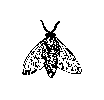
\includegraphics{fly}
% \caption{A sample black and white graphic.}
% \end{figure}

% \begin{figure}
% 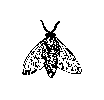
\includegraphics[height=1in, width=1in]{fly}
% \caption{A sample black and white graphic
% that has been resized with the \texttt{includegraphics} command.}
% \end{figure}


% As was the case with tables, you may want a figure that spans two
% columns.  To do this, and still to ensure proper ``floating''
% placement of tables, use the environment \textbf{figure*} to enclose
% the figure and its caption.  And don't forget to end the environment
% with \textbf{figure*}, not \textbf{figure}!

% \begin{figure*}
% 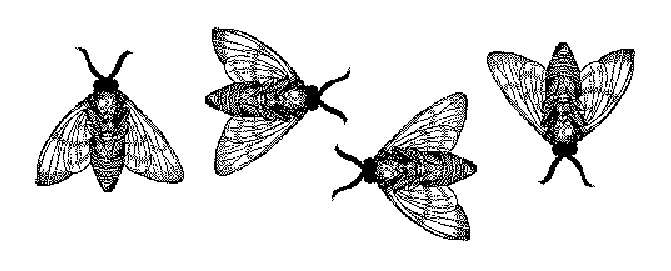
\includegraphics{flies}
% \caption{A sample black and white graphic
% that needs to span two columns of text.}
% \end{figure*}


% \begin{figure}
% 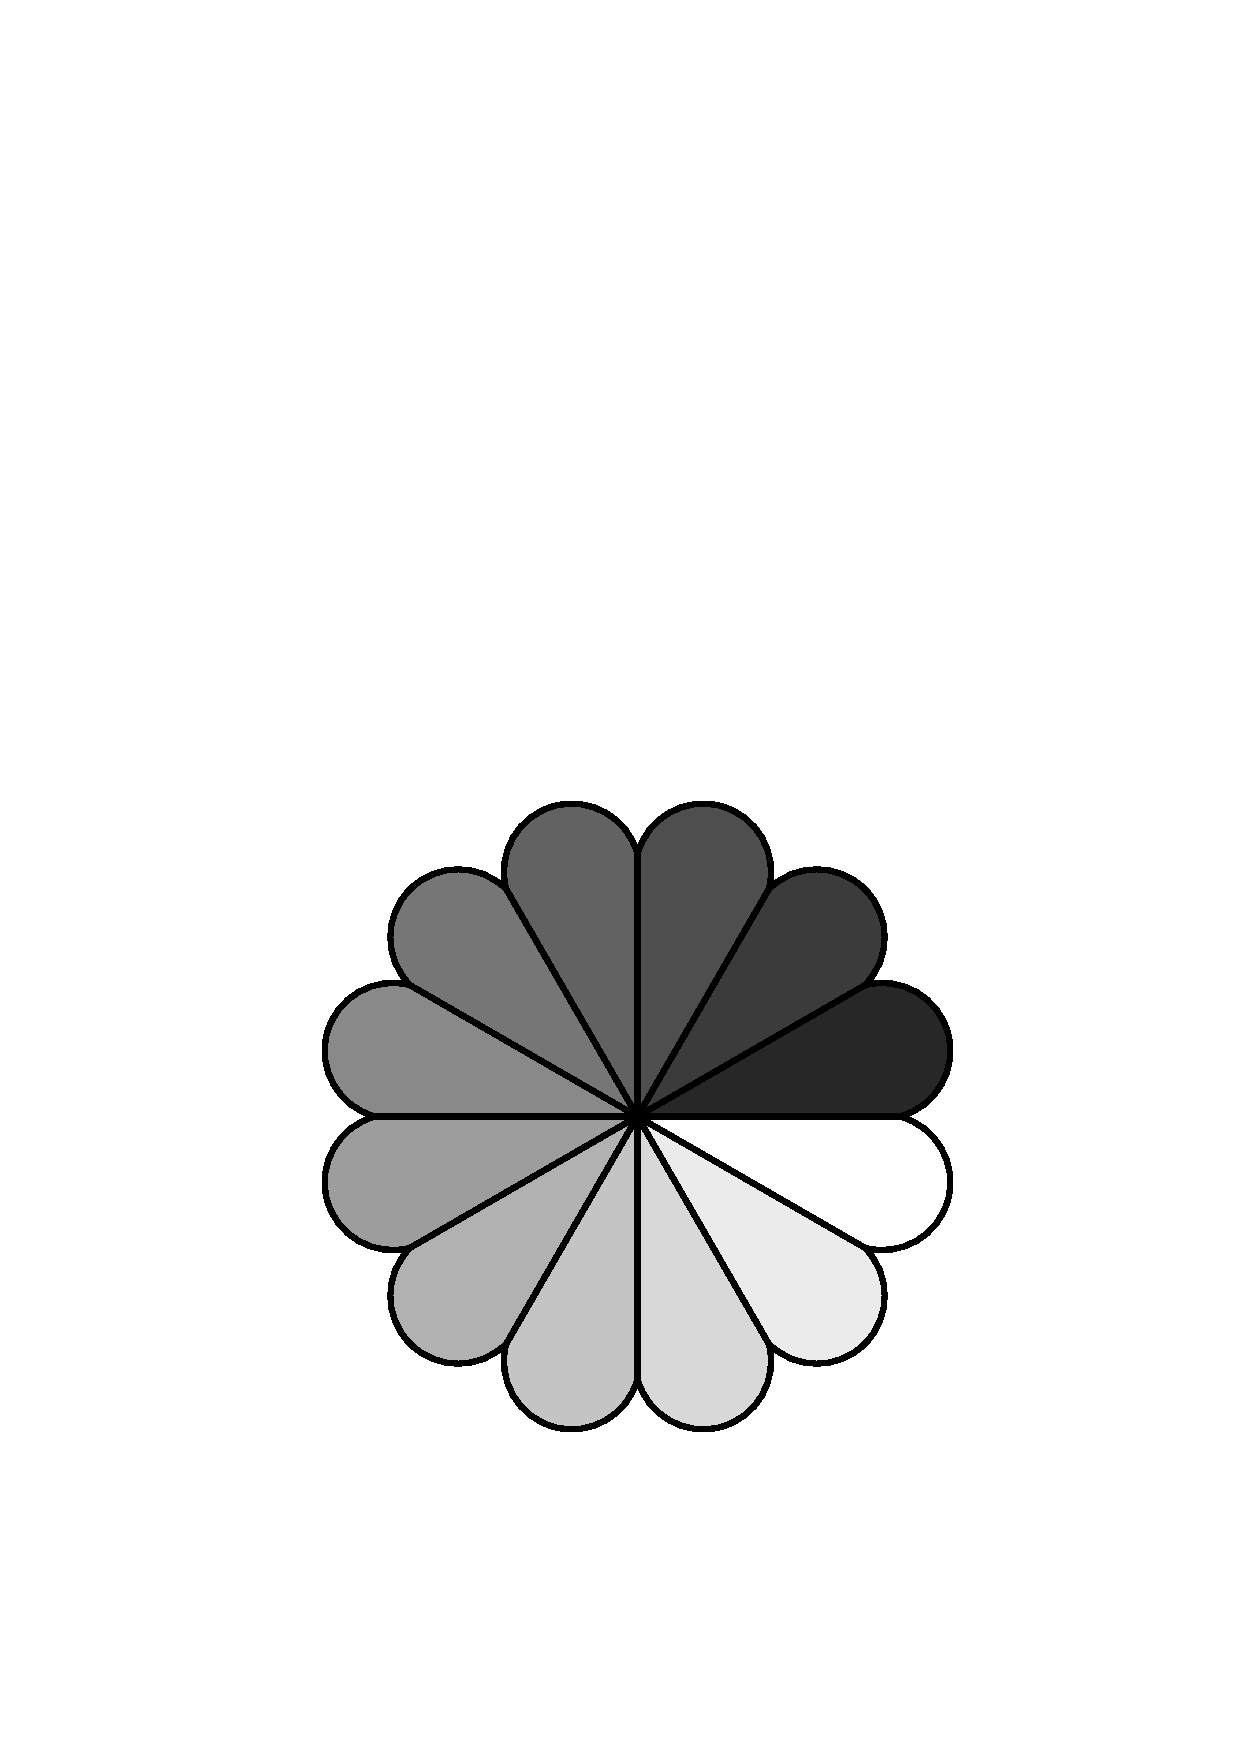
\includegraphics[height=1in, width=1in]{rosette}
% \caption{A sample black and white graphic that has
% been resized with the \texttt{includegraphics} command.}
% \end{figure}

% \subsection{Theorem-like Constructs}

% Other common constructs that may occur in your article are the forms
% for logical constructs like theorems, axioms, corollaries and proofs.
% ACM uses two types of these constructs:  theorem-like and
% definition-like.

% Here is a theorem:
% \begin{theorem}
%   Let $f$ be continuous on $[a,b]$.  If $G$ is
%   an antiderivative for $f$ on $[a,b]$, then
%   \begin{displaymath}
%     \int^b_af(t)\,dt = G(b) - G(a).
%   \end{displaymath}
% \end{theorem}

% Here is a definition:
% \begin{definition}
%   If $z$ is irrational, then by $e^z$ we mean the
%   unique number that has
%   logarithm $z$:
%   \begin{displaymath}
%     \log e^z = z.
%   \end{displaymath}
% \end{definition}

% The pre-defined theorem-like constructs are \textbf{theorem},
% \textbf{conjecture}, \textbf{proposition}, \textbf{lemma} and
% \textbf{corollary}.  The pre-defined de\-fi\-ni\-ti\-on-like constructs are
% \textbf{example} and \textbf{definition}.  You can add your own
% constructs using the \textsl{amsthm} interface~\cite{Amsthm15}.  The
% styles used in the \verb|\theoremstyle| command are \textbf{acmplain}
% and \textbf{acmdefinition}.

% Another construct is \textbf{proof}, for example,

% \begin{proof}
%   Suppose on the contrary there exists a real number $L$ such that
%   \begin{displaymath}
%     \lim_{x\rightarrow\infty} \frac{f(x)}{g(x)} = L.
%   \end{displaymath}
%   Then
%   \begin{displaymath}
%     l=\lim_{x\rightarrow c} f(x)
%     = \lim_{x\rightarrow c}
%     \left[ g{x} \cdot \frac{f(x)}{g(x)} \right ]
%     = \lim_{x\rightarrow c} g(x) \cdot \lim_{x\rightarrow c}
%     \frac{f(x)}{g(x)} = 0\cdot L = 0,
%   \end{displaymath}
%   which contradicts our assumption that $l\neq 0$.
% \end{proof}

% \section{Conclusions}
% This paragraph will end the body of this sample document.
% Remember that you might still have Acknowledgments or
% Appendices; brief samples of these
% follow.  There is still the Bibliography to deal with; and
% we will make a disclaimer about that here: with the exception
% of the reference to the \LaTeX\ book, the citations in
% this paper are to articles which have nothing to
% do with the present subject and are used as
% examples only.
% %\end{document}  % This is where a 'short' article might terminate



% \appendix
% %Appendix A
% \section{Headings in Appendices}
% The rules about hierarchical headings discussed above for
% the body of the article are different in the appendices.
% In the \textbf{appendix} environment, the command
% \textbf{section} is used to
% indicate the start of each Appendix, with alphabetic order
% designation (i.e., the first is A, the second B, etc.) and
% a title (if you include one).  So, if you need
% hierarchical structure
% \textit{within} an Appendix, start with \textbf{subsection} as the
% highest level. Here is an outline of the body of this
% document in Appendix-appropriate form:
% \subsection{Introduction}
% \subsection{The Body of the Paper}
% \subsubsection{Type Changes and  Special Characters}
% \subsubsection{Math Equations}
% \paragraph{Inline (In-text) Equations}
% \paragraph{Display Equations}
% \subsubsection{Citations}
% \subsubsection{Tables}
% \subsubsection{Figures}
% \subsubsection{Theorem-like Constructs}
% \subsubsection*{A Caveat for the \TeX\ Expert}
% \subsection{Conclusions}
% \subsection{References}
% Generated by bibtex from your \texttt{.bib} file.  Run latex,
% then bibtex, then latex twice (to resolve references)
% to create the \texttt{.bbl} file.  Insert that \texttt{.bbl}
% file into the \texttt{.tex} source file and comment out
% the command \texttt{{\char'134}thebibliography}.
% % This next section command marks the start of
% % Appendix B, and does not continue the present hierarchy
% \section{More Help for the Hardy}

% Of course, reading the source code is always useful.  The file
% \path{acmart.pdf} contains both the user guide and the commented
% code.

% \begin{acks}
%   The authors would like to thank Dr. Yuhua Li for providing the
%   matlab code of  the \textit{BEPS} method. 

%   The authors would also like to thank the anonymous referees for
%   their valuable comments and helpful suggestions. The work is
%   supported by the \grantsponsor{GS501100001809}{National Natural
%     Science Foundation of
%     China}{http://dx.doi.org/10.13039/501100001809} under Grant
%   No.:~\grantnum{GS501100001809}{61273304}
%   and~\grantnum[http://www.nnsf.cn/youngscientsts]{GS501100001809}{Young
%     Scientsts' Support Program}.

% \end{acks}
